\section{Охрана труда}
\subsection{Введение}

В процессе создания ПО эксплуатирующий его персонал подвергается воздействию ряда опасных и вредных факторов, среди которых можно перечислить электромагнитное излучение, отражённый свет, блики и шум.

В данном разделе рассматриваются основные виды опасных и вредных факторов, и на основе их анализа вырабатываются требования к рабочему помещению на основе требований СанПиН.

\subsection{Анализ опасных и вредных факторов}
\subsubsection{Микроклимат}

Работа программиста относится к категории 1а (не предполагает физических усилий). Поэтому нормы микроклимата определяются таблицей ~\ref{table:climate}.

\begin{table}[h]
  \begin{tabu}{|X[c]|X[c]|X[c]|X[c]|}\hline
    & \shortstack{Температура\\воздуха, $^\circ \mathrm{C}$} 
    & \shortstack{Отн. влажность\\воздуха, \%}
    & \shortstack{Скорость движ.\\воздуха, м/с}\\\hline 
    Холодный & 22-24 & 40-60 & 0,1 \\\hline
    Теплый & 23-25 & 40-60 & 0,1 \\\hline
  \end{tabu}
  \caption{Оптимальные нормы микроклимата}
  \label{table:climate}
\end{table}

Для борьбы с запылённостью помещения, являющейся ещё более вредным фактором в сочетании с электростатическими полями ПК, предусмотрено использование системы кондиционирования. Использование подобной системы также позволяет регулировать показатели температуры, влажности и скорости движения воздуха. 

Нормы СанПиН 2.2.4.1294-03 определяют уровни содержания ионов
в воздухе (таблица ~\ref{table:ions}). Для обеспечения требуемых уровней предусмотрено использование системы ионизации воздуха.

\begin{table}[h]
  \begin{tabu}{|X[c]|X[c]|X[c]|}  
    \hline
    \multirow{2}{*}{Уровни} & \multicolumn{2}{|c|}{Число ионов в 1 см куб. воздуха} \\\cline{2-3}
    & $n^+$ & $n^-$\\\hline
    Минимально необходимые & 400 & 600 \\\hline
    Оптимальные & 1500-3000 & 3000-5000 \\\hline
    Предельно допустимые & 50000 & 50000 \\\hline
  \end{tabu}
  \caption{Уровни ионизации воздуха помещений при работе на ПЭВМ}
  \label{table:ions}
\end{table}


\subsubsection{Шум}

При разработке программного обеспечения внутренними источниками шума являются вентиляторы, а также принтеры и другие периферийные устройства ЭВМ. Внешние источники шума – прежде всего, шум с улицы и из соседних помещений. Постоянные внешние источники шума, превышающего нормы, отсутствуют. План помещения с источниками света дан на рисунке ~\ref{fig:srvplan}. Габариты помещения даны в таблице ~\ref{table:srvsize}. Вспомогательные расчётные параметры даны в таблице ~\ref{table:srvparams}. Характеристики источников шума (положение, расстояние, уровни звуковой мощности и расчётная площадь) и спектральные параметры помещения даны в таблице ~\ref{table:srvnoisesrc}. Расчётные и предельные уровни звуковой интенсивности для напольных источников шума даны в таблице ~\ref{table:srvnoiseint}. Расчётный и предельный спектры даны на рисунке ~\ref{fig:srvspectrum}.

Как видно из расчётов, расчётный спектр превышает предельно допустимый уровень шума. Определено, что увеличение Ri - расстояния до источников шума
слабо влияет на уровень шума. Изменение габаритов комнаты, однако, может в значительной мере повлиять на уровень шума в помещении в
целом, но по результатам расчётов также не позволяет снизить его до допустимых значений. Действенным защитным мероприятием в этом
Случае будет являться введение звукоизоляции, акустическая обработка помещения. Также возможно вынесение рабочих мест за пределы зашумлённого помещения, где, в случае оборудования данного помещения звукопоглощающими покрытиями (прорезиненные ковры, пористые покрытия, ширмы, многослойные покрытия с воздушным промежутком), уровни звукового давления будут допустимыми.

\begin{figure}[h]
  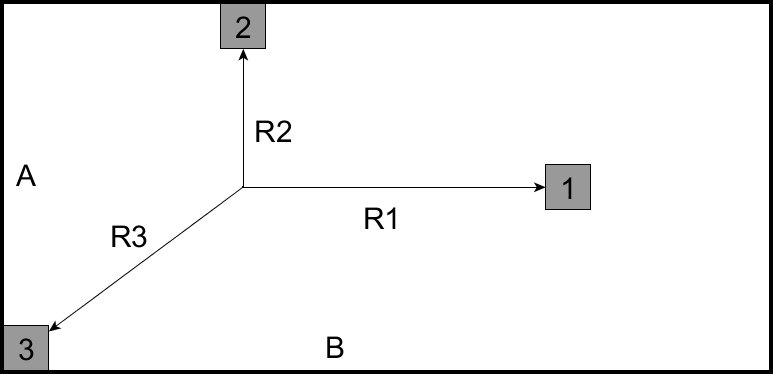
\includegraphics[width=\textwidth]{img/srvplan.png}
  \caption{Схема расположения расчётной точки относительно источников шума}
  \label{fig:srvplan} 
\end{figure}

\begin{table}[h]
\centering
\begin{minipage}[t]{.45\textwidth}
  \centering
  \begin{tabu}{|X[c]|X[c]|}\hline
    Длина(А) & 15 \\\hline
    Ширина(В) & 30 \\\hline
    Высота(С) & 4 \\\hline
    Объем(V) & 1800 \\\hline
  \end{tabu}
  \caption{Габариты комнаты}
  \label{table:srvsize}
\end{minipage}
\hfil
\begin{minipage}[t]{.45\textwidth}
  \centering
  \begin{tabu}{|X[c]|X[c]|}\hline
    Ф & 1 \\\hline
    Х & 1 \\\hline
    B1000 & 90 \\\hline
    æ & 1 \\\hline
  \end{tabu}
  \caption{Вспомогательные пар-ры}
  \label{table:srvparams}
\end{minipage}
\end{table}

\begin{table}[h]
  \begin{tabu}{|c|c|c|c|c|c|c|c|c|c|c|X[c]|}
    \hline
    \multirow{2}{*}{№} &
    \multirow{2}{*}{\shortstack{Тип\\монтажа}} &    
    \multirow{2}{*}{$R_i$} & 
    \multicolumn{8}{|c|}{Ур-нь звуковой мощности, Lw для окт. полос} &
    \multirow{2}{*}{S} \\\cline{4-11}      
     & & & 63 & 125 & 250 & 500 & 1000 & 2000 & 4000 & 8000 & \\\hline
    1 & подвешен & 9 & 81 & 82 & 83 & 84 & 83 & 81 & 80 & 77 & 508 \\\hline
    2 & на полу & 9 & 90 & 91 & 98 & 99 & 97 & 93 & 91 & 86 & 254 \\\hline
    3 & на полу & 9 & 84 & 82 & 84 & 91 & 94 & 94 & 91 & 91 & 127 \\\hline 
    
    \multicolumn{2}{c}{} & \multicolumn{9}{|c|}{Спектральные параметры помещения} & \multicolumn{1}{c}{}\\\cline{3-11}
    \multicolumn{2}{c|}{} & y & 0,5 & 0,5 & 0,55 & 0,7 & 1 & 1,6 & 3 & 6\\\cline{3-11}
    \multicolumn{2}{c|}{} & B & 45 & 45 & 49,5 & 63 & 90 & 144 & 270 & 540\\\cline{3-11}
  \end{tabu}
  \caption{Параметры источников звука и спектральные параметры помещения}
  \label{table:srvnoisesrc}
\end{table}

\begin{table}[h]
  \begin{tabu}{|X[c]|X[c]|X[c]|X[c]|X[c]|X[c]|X[c]|X[c]|X[c]||}
    \hline
    № &
    \multicolumn{8}{|c|}{Уровни звуковой интенсивности, Lj}\\\hline
    2 & 79,68 & 80,68 & 87,28 & 87,29 & 83,85 & 78,01 & 73,73 & 66,55 \\\hline
    3 & 73,86 & 71,86 & 73,48 & 79,53 & 81,19 & 79,52 & 74,56 & 72,84 \\\hline
    $Lj_{sum}$ & 80,69 & 81,21 & 87,46 & 87,96 & 85,73 & 81,84 & 77,17 & 73,75 \\\hline
    $L_{lim}$ & 83 & 74 & 68 & 63 & 60 & 57 & 55 & 54 \\\hline
  \end{tabu}
  \caption{Расчётные и предельные уровни звуковой интенсивности}
  \label{table:srvnoiseint}
\end{table}

\begin{figure}[h]
  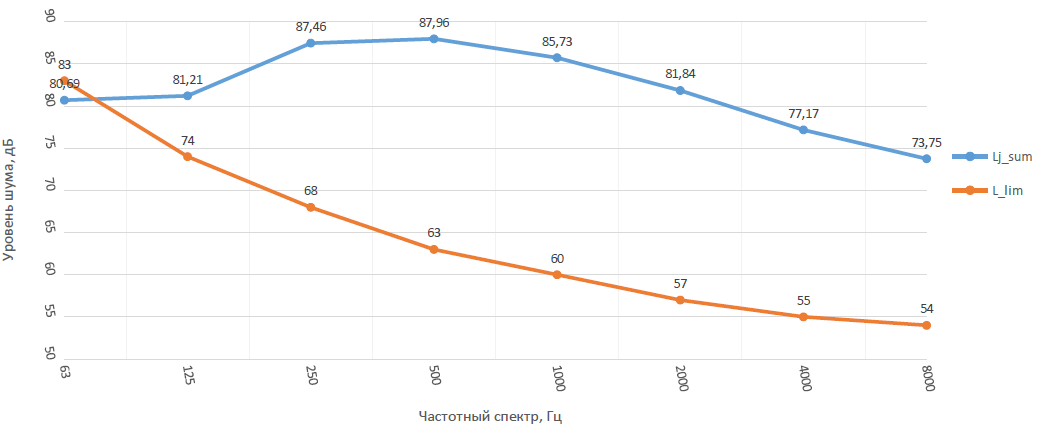
\includegraphics[width=\textwidth]{img/spectrum.png}
  \caption{Расчётный и предельный спектры}
  \label{fig:srvspectrum}
\end{figure}

\subsubsection{Электробезопасность}

При работе с ПК работник подвергается повышенному риску удара электрическим током, поскольку проводит много времени около корпуса компьютера. Для работы за компьютером он должен быть оборудован защитным заземлением в соответствии с техническими требованиями.

\subsubsection{Свет}

Одним из основных опасных и вредных факторов при работе за компьютером является повышенная нагрузка на глаза. Отсюда следующие общие требования:
\begin{itemize}
	\item Окна должны быть ориентированы преимущественно на север и северо-восток
	\item Коэффициенты отражения должны составлять 0,7-0,8 для потолка, 0,5-0,6 для стен и 0,3-0,5 для пола.
	\item Окна должны быть оборудованы средствами регулирования (жалюзи, занавеси)
\end{itemize}

Требования к освещению на рабочих местах представлены в таблице ~\ref{table:lightreq}.
\begin{table}[h]
  \begin{tabu}{|X[c]|X[c]|}\hline
    Освещенность на поверхности стола & 300 - 500 лк. \\\hline
    Освещенность поверхности экрана & <300 лк. \\\hline
    \shortstack{Яркость светящихся поверхностей\\(окна, светильники и др.),\\ находящихся в поле зрения} & 200 кд/м2. \\\hline
    Показатель ослепленности & <20 \\\hline
    Яркость светильников общего освещения & <200 кд/м2 \\\hline
    Коэффициент запаса (Кз) & 1.4 \\\hline
    Коэффициент пульсации & 5\% \\\hline
  \end{tabu}
  \caption{Требования к освещению на рабочих местах с ПК}
  \label{table:lightreq}
\end{table}

Расчёт освещения в соответствии с планом помещения был произведён в программе DIALux 4.12.01. План помещения и ведомость объектов даны на рисунке ~\ref{fig:lightplan} и таблице ~\ref{table:lightitemlist} соответственно. Паспорт светильника предоставлен на рисунке ~\ref{fig:lightpassport}. Данные светотехнических результатов расчёта даны на рисунке ~\ref{fig:lighttechres}. План помещения с указанием изолиний освещённости и ведомость светильников даны на рисунке ~\ref{fig:lightiso}. 3D-визуализация помещения дана на рисунке ~\ref{fig:light3d}.

\begin{figure}[h]
  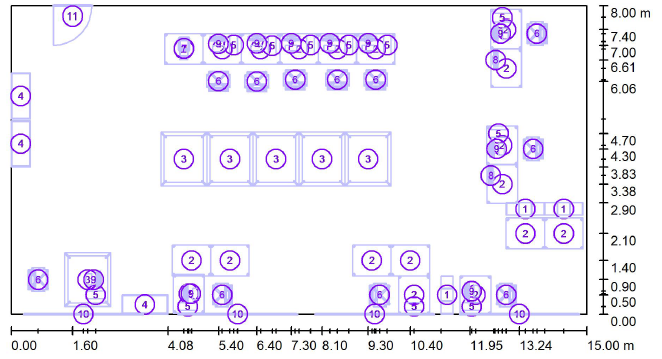
\includegraphics[width=\textwidth]{img/lightplan}
  \caption{План помещения}
  \label{fig:lightplan}
\end{figure}

\begin{table}[h]
  \begin{tabu}{|X[c]|X[c]|X[c]|}\hline
    № & Шт. & Обозначение \\\hline
    1 & 3 & 100x200 квадрат \\\hline
    2 & 19 & 100x80 стандарт. \\\hline
    3 & 6 & 120x140 дельта \\\hline
    4 & 3 & 120x200 2двери \\\hline
    5 & 11 & компьютер t \\\hline
    6 & 11 & офисный стул 1 \\\hline
    7 & 1 & принтер t \\\hline
    8 & 2 & экран TFT \\\hline
    9 & 10 & экран TFT и клавиатура \\\hline
    10 & 4 & Окно \\\hline
    11 & 1 & Дверь \\\hline
  \end{tabu} 
  \caption{Ведомость объектов}
  \label{table:lightitemlist}
\end{table}

\begin{figure}[h]
  \centering
  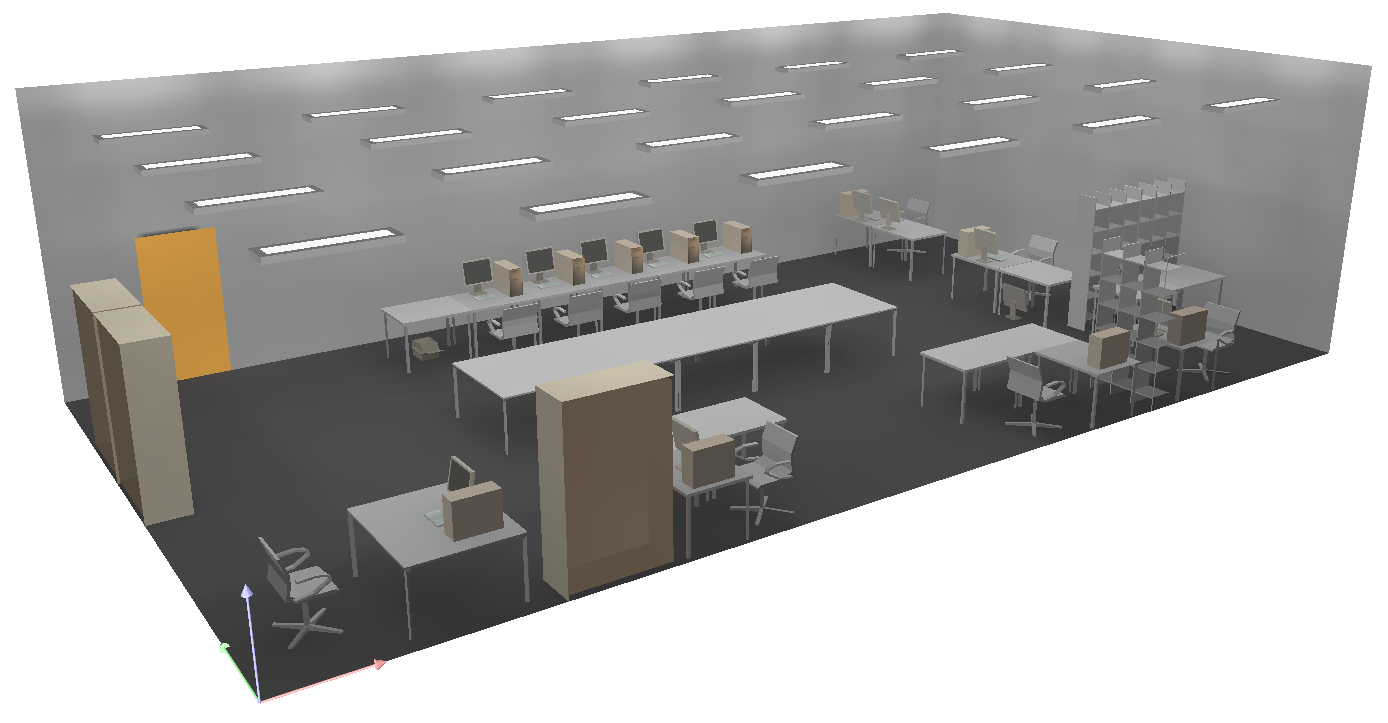
\includegraphics[width=\textwidth]{img/light3d}
  \caption{3D-визуализация помещения}
  \label{fig:light3d}
\end{figure}

\clearpage
\begin{figure}[h]
  \centering
  \includegraphics[page=3,height=.8\textheight]{img/lightcalc}
  \caption{Паспорт светильника}
  \label{fig:lightpassport}
\end{figure}

\clearpage
\begin{figure}[h]
  \centering
  \includegraphics[page=8,height=.8\textheight]{img/lightcalc}
  \caption{Светотехнические результаты}
  \label{fig:lighttechres}
\end{figure}

\clearpage
\begin{figure}[h]
  \centering
  \includegraphics[page=4,height=.8\textheight]{img/lightcalc}
  \caption{Резюме светового расчёта}
  \label{fig:lightiso}
\end{figure}
\clearpage

\subsection{Вывод}

В результате анализа санитарных норм в соответствии с ними в данном разделе были выработаны требования к рабочему помещению. На основании данных требований был спланирован интерьер помещения с указанием расположения светоизлучающих элементов. Спланированное помещение соответствует условиям по безопасности помещений и охране труда.

Был проведён расчёт освещения для данного помещения в программе DIALux. Были установлены мощность освещения и изолиниями показаны уровни освещения во всех точках помещения.

В соответствии с вариантом индивидуального задания был произведён расчёт уровней шума в помещении серверной для каждой октавной полосы из расчётных. Были предложены рекомендации по снижению уровня шума в помещении с серверами и по разделению помещения на рабочее и служебное, с целью сокращения времени пребывания людей в помещении с повышенным уровнем шума.